\section{$\mu^+\to e^+e^-e^+$}
\label{mutoeee}

The current bound on the $\mu^+\to e^+e^-e^+$ decay has been set by the SINDRUM experiment at PSI~\cite{Bellgardt:1987du}. No signal was observed, and a limit ${\cal B}(\mu^+\to e^+e^-e^+) < 1\times 10^{-12}$ was set, assuming a decay model with a constant matrix element. This limit was essentially driven by the number of stopped muons, the background from $\mu^+\to e^+e^-e^+ \nu_e \bar\nu_\mu$ decays remaining negligible. 
The Mu3e experiment~\cite{Blondel:2013ia} has been proposed to improve this bound by four orders of magnitude, reaching a single event sensitivity (SES) at the level of $10^{-16}$. The experiment consists of a cylindrical silicon tracker instrumented with a time of flight system. We present a study of a similar setup, and discuss the requirements needed to improve the sensitivity by an order of magnitude with respect to Mu3e.
 
The proposed detector consists of a silicon tracker surrounding an active target. The tracker is composed of 6 layers of cylindrical silicon detectors positioned at radii of 2, 3, 8, 9, 15, 16 cm with respect to the center of the target. 
The silicon modules are modeled in the same way as those in $\mu\to e\gamma$
detector described in the previous section.
%%Each layer is formed of 50 $\mu$m thick double-sided striplets silicon sensors mounted on 50 $\mu$m of kapton. The hit spatial resolution is modeled as a sum of two components with resolutions of 8 $\mu$m and 20 $\mu$m, and a hit efficiency of 90\%. 
The target is made of two hollow cones of silicon pixel detectors, assuming a pixel size of 50 $\mu$m by 50 $\mu$m. The cone length and radius are set to 5 cm and 1 cm, respectively. Although not included, a time-of-flight system should be installed as well. We assume a time resolution of 250 ps, averaging the values quoted by Mu3e. The apparatus is displayed in Fig.~\ref{Fig::mu3e}, together with a simulated $\mu^+ \rightarrow e^+e^-e^+$ event.

We generate $\mu^+ \rightarrow e^+e^-e^+$ events according to phase space, and constrain the tracks to originate from the same pixel in the active target. To further improve the resolution, we require the probability of the constrained fit to be greater than 1\%, and the reconstructed muon momentum less than $1 ~\Mev$. The absolute value of the cosine of the polar angle of each electron must also be less than 0.9. The resulting $e^+e^-e^+$ invariant mass distribution is shown in Fig.~\ref{Fig::mu3e}, and peaks sharply at the muon mass. We extract the resolution by fitting this spectrum with a double-sided Crystal Ball function (a Gaussian with power-law tails on both sides). The Gaussian resolution is found to be 0.3~\Mev\. To investigate the contribution of the active target to the resolution, we performed alternative fits removing the geometric constraints, or taking the vertex position by considering all points from tracks intercepting the target, and choosing the one minimizing the $\chi^2$ of the constrained fit. While we observe an improvement compared to the unconstrained fit, the second method yields similar signal resolution. However, the active target provides a better estimate of impact parameters of the tracks, improving background rejection.

The signal efficiency is found to be 27\%. To achieve a SES at the level of $5\times\sim 10^{-18}$ after a 3-year run (100\% duty cycle), a stop muon rate of the order of $8\times 10^{9}$ is needed. For comparison, the estimated Mu3e stop muon rate at the HiMB beam at PSI is expected to be $2\times 10^{9}$.   

For the purpose of estimating background contributions, we define a signal window as $ 104.9 < m_{eee} < 106.5 ~\Mev$, containing approximately 90\% of the signal. The irreducible background arise from $\mu \rightarrow e^+e^-e^+ \nu\bar\nu$ events where the two neutrinos carry almost no energy. We estimate its contribution to be about 7.5 events by convolving the branching fraction with the resolution function and integrating in the signal region, as shown in Figure~\ref{Fig::mu3e2}. We assume an efficiency of 27\%. However, this background depends strongly on the tail resolution, and small improvements translate into large background reductions. For example, decreasing the thickness of the silicon sensors and the supporting kapton structure by 20\% (40\%) reduces the background down to $\sim 4$ ($\sim 1$) events. Additional improvements of the reconstruction algorithms might further ameliorate the resolution and reduce this contamination.

\begin{figure}[htb]
\begin{center}
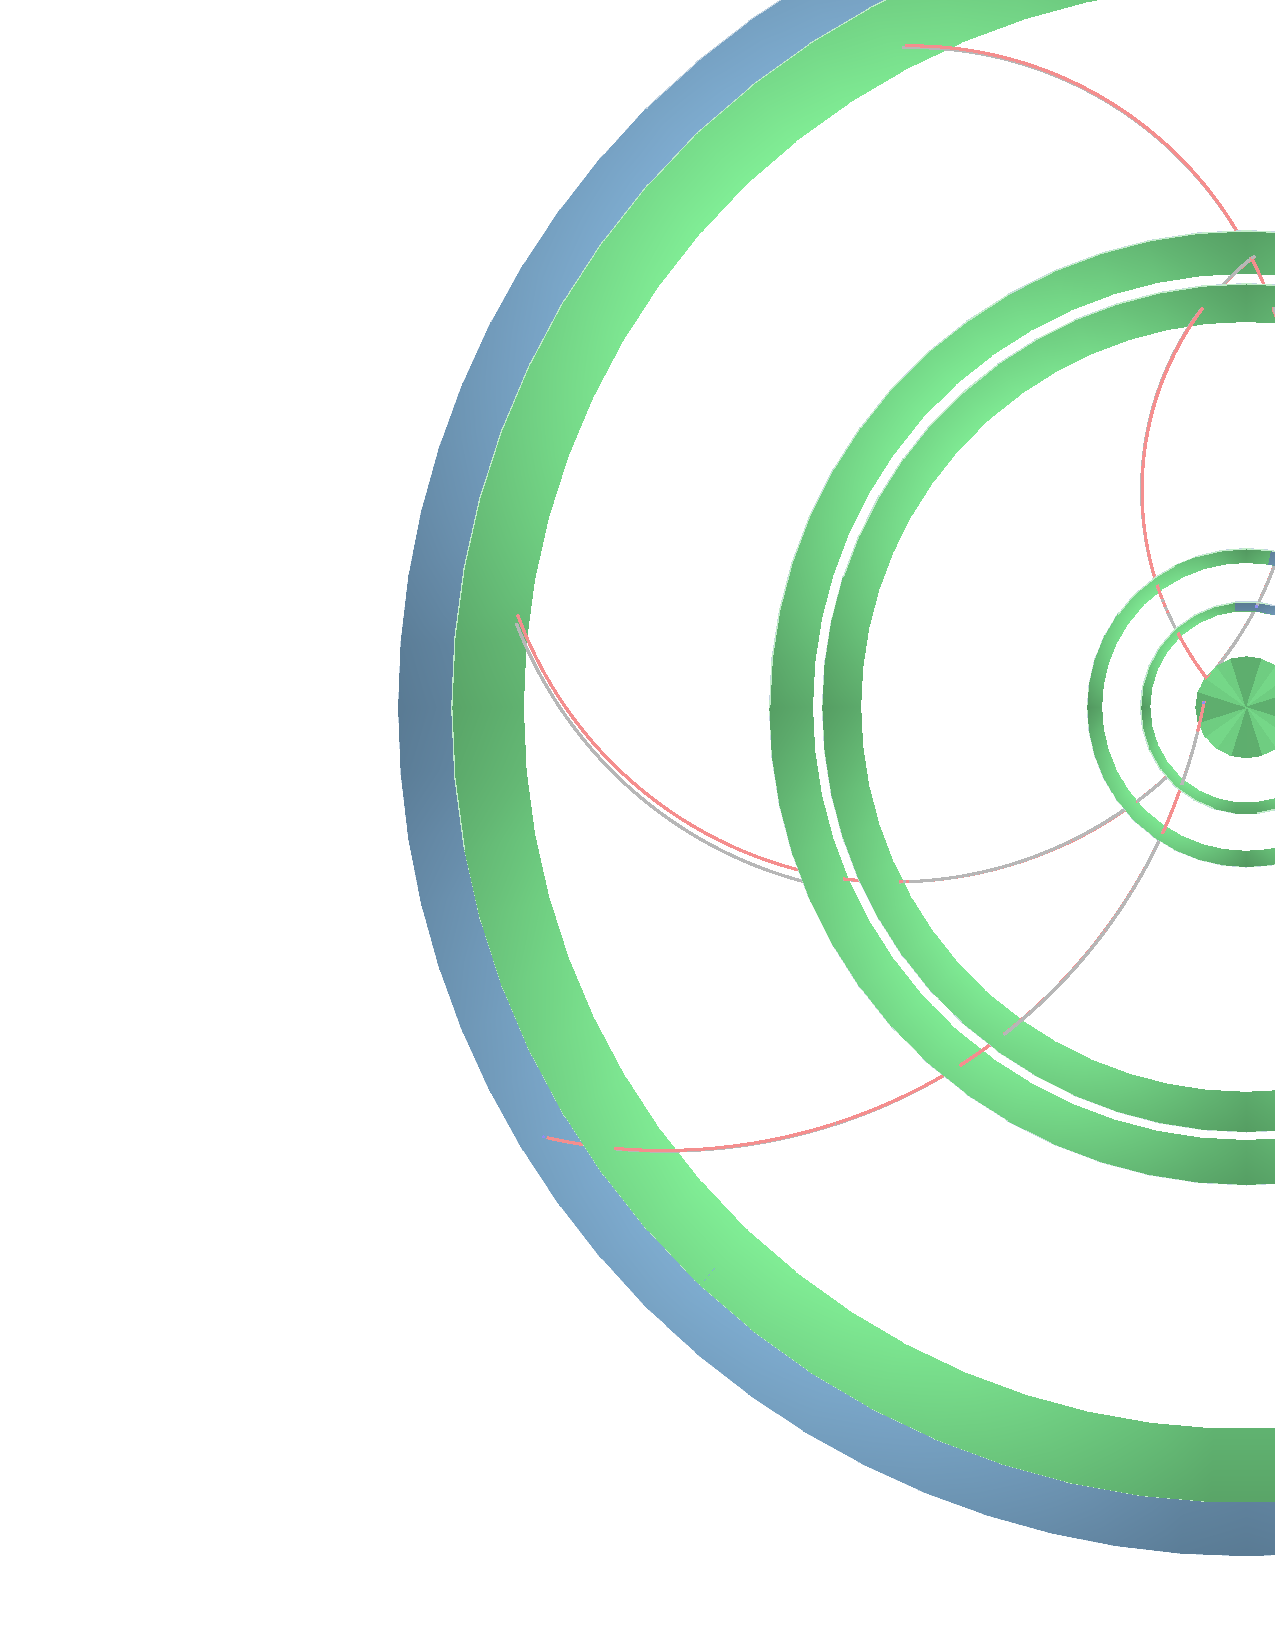
\includegraphics[width=0.45\textwidth]{Figures/mu3e-event.pdf}
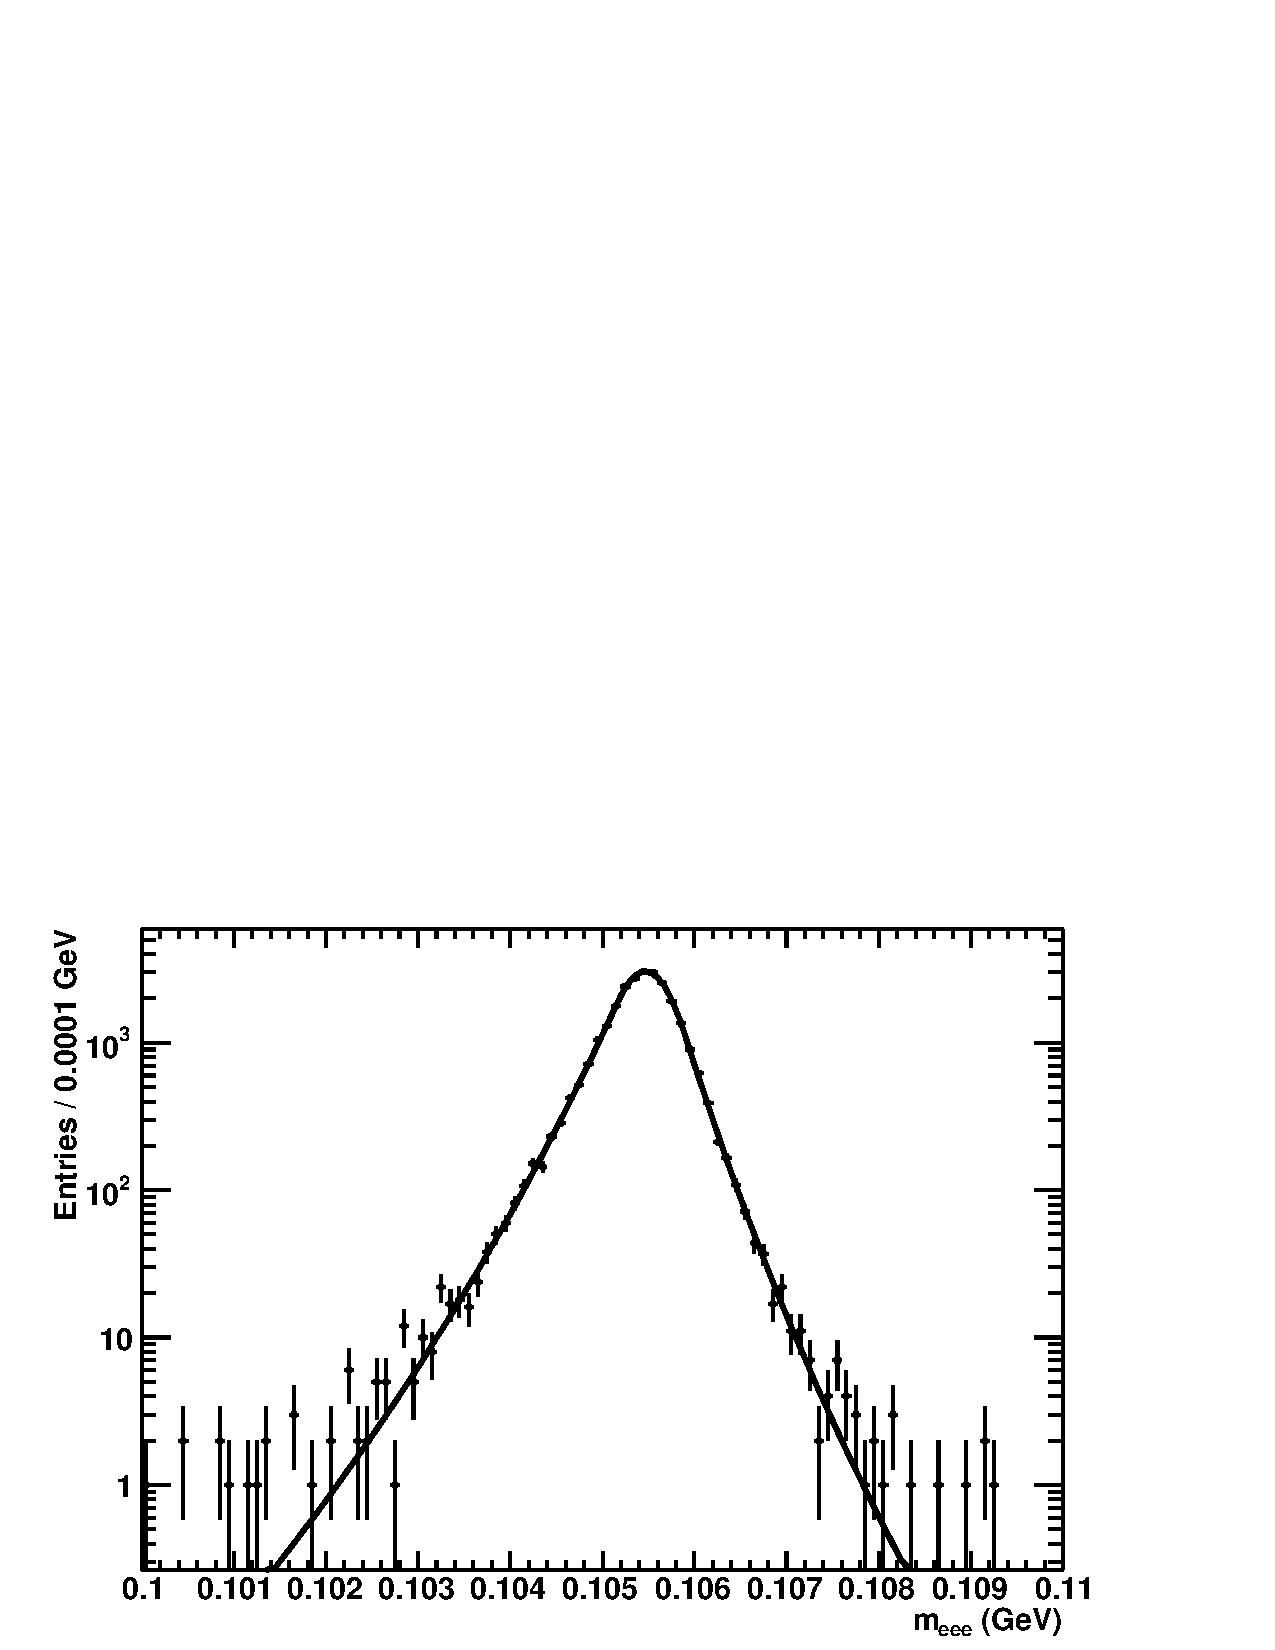
\includegraphics[width=0.45\textwidth]{Figures/mu3e-resoFit.pdf}
\end{center}
\caption{Left: Display of the experimental setup, together with a simulated $\mu^+ \rightarrow e^+e^-e^+$ event. 
Right:  The $e^+e^-e^+$ invariant mass distribution after all selection criteria are applied fitted by a 
sum of two Gaussian functions.}
\label{Fig::mu3e}
\end{figure}

\begin{figure}[htb]
\begin{center}
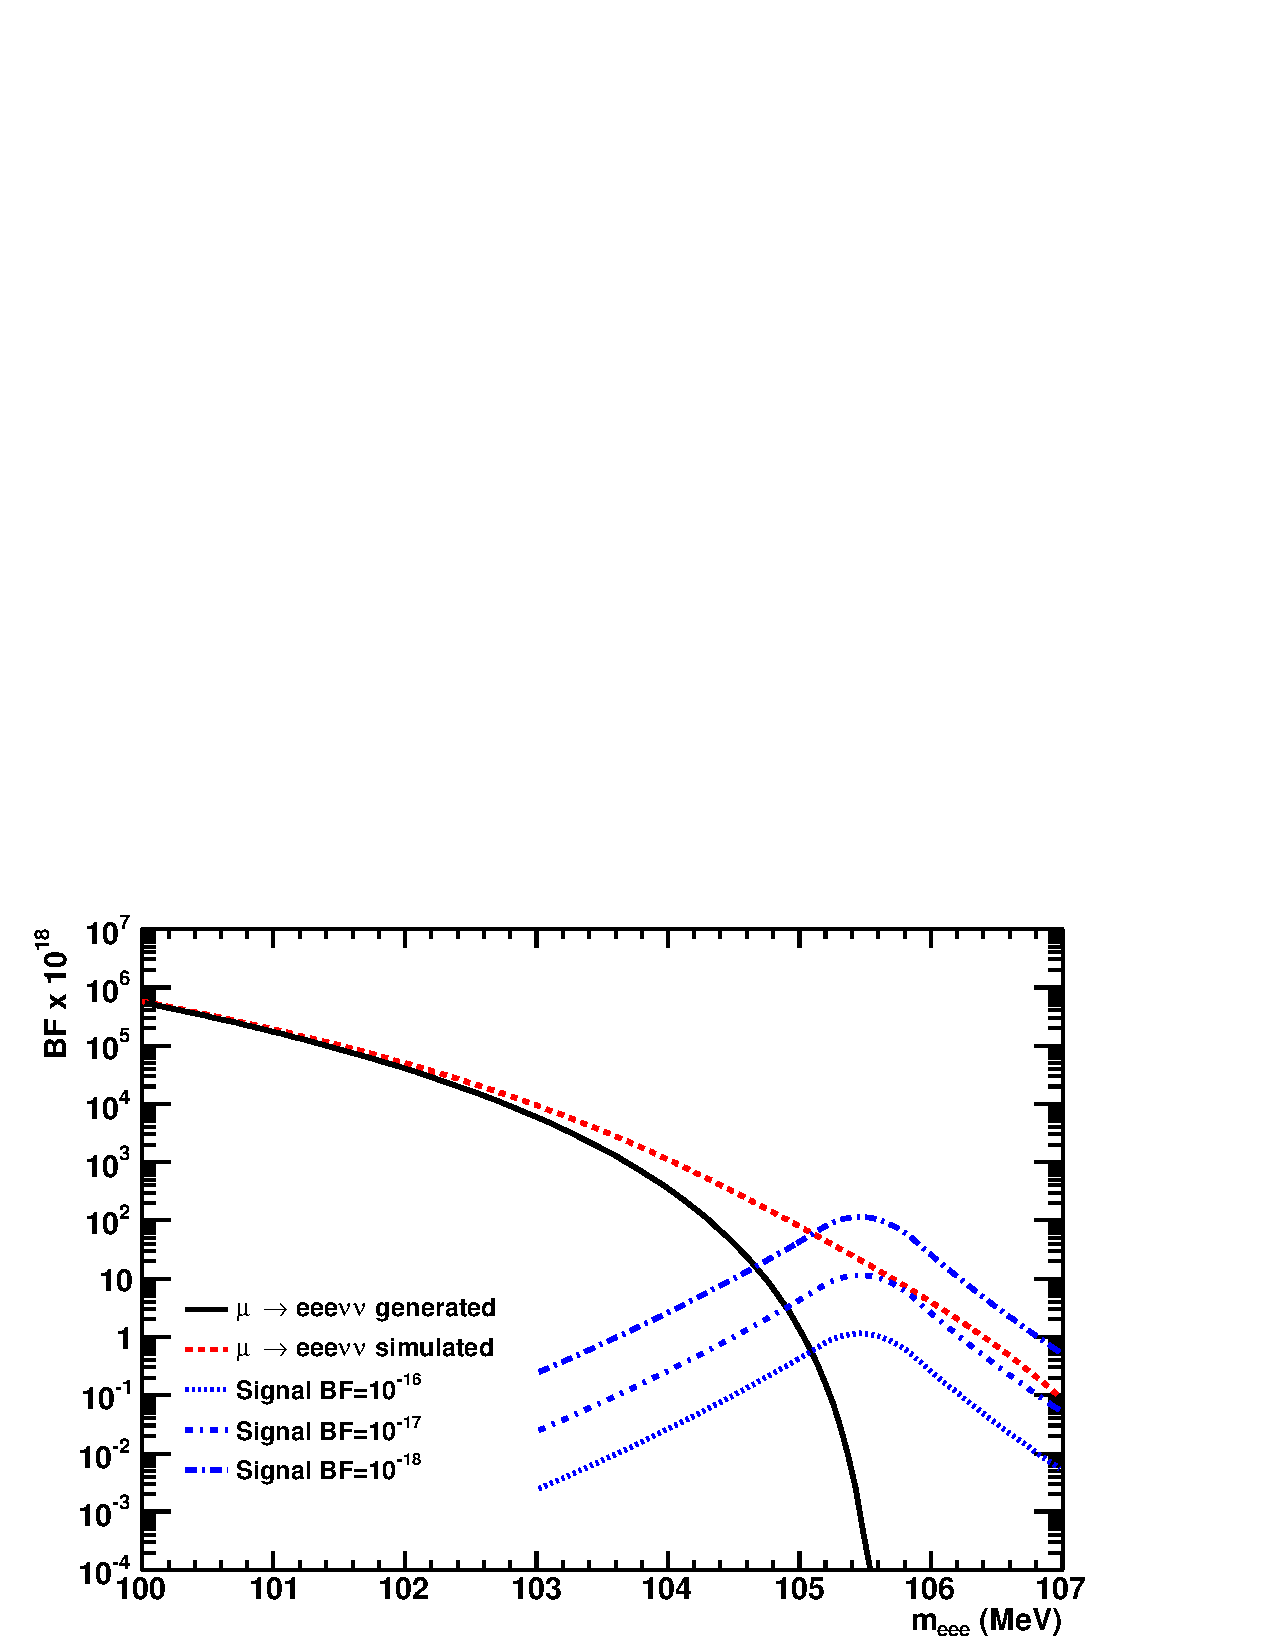
\includegraphics[width=0.45\textwidth]{Figures/mu3e-irr.pdf}
%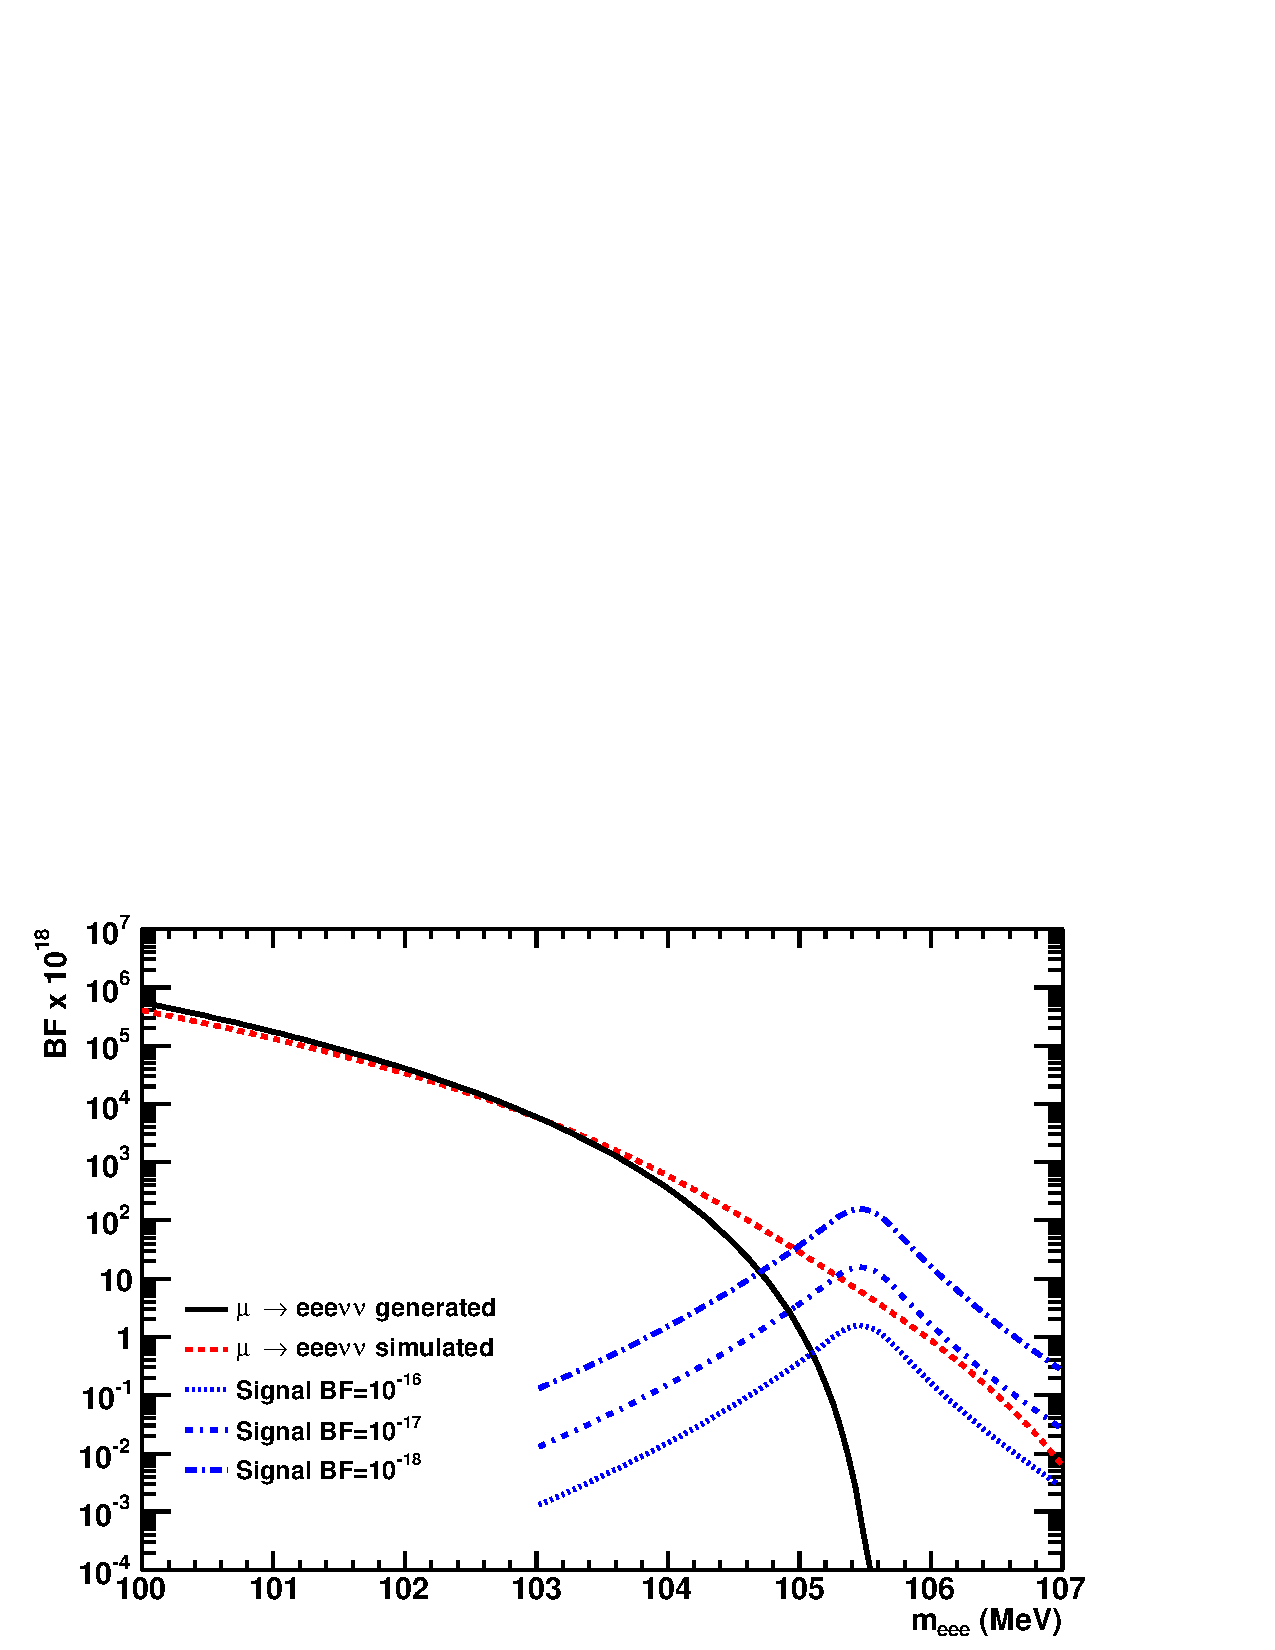
\includegraphics[width=0.45\textwidth]{Figures/mu3e-irr2.pdf}
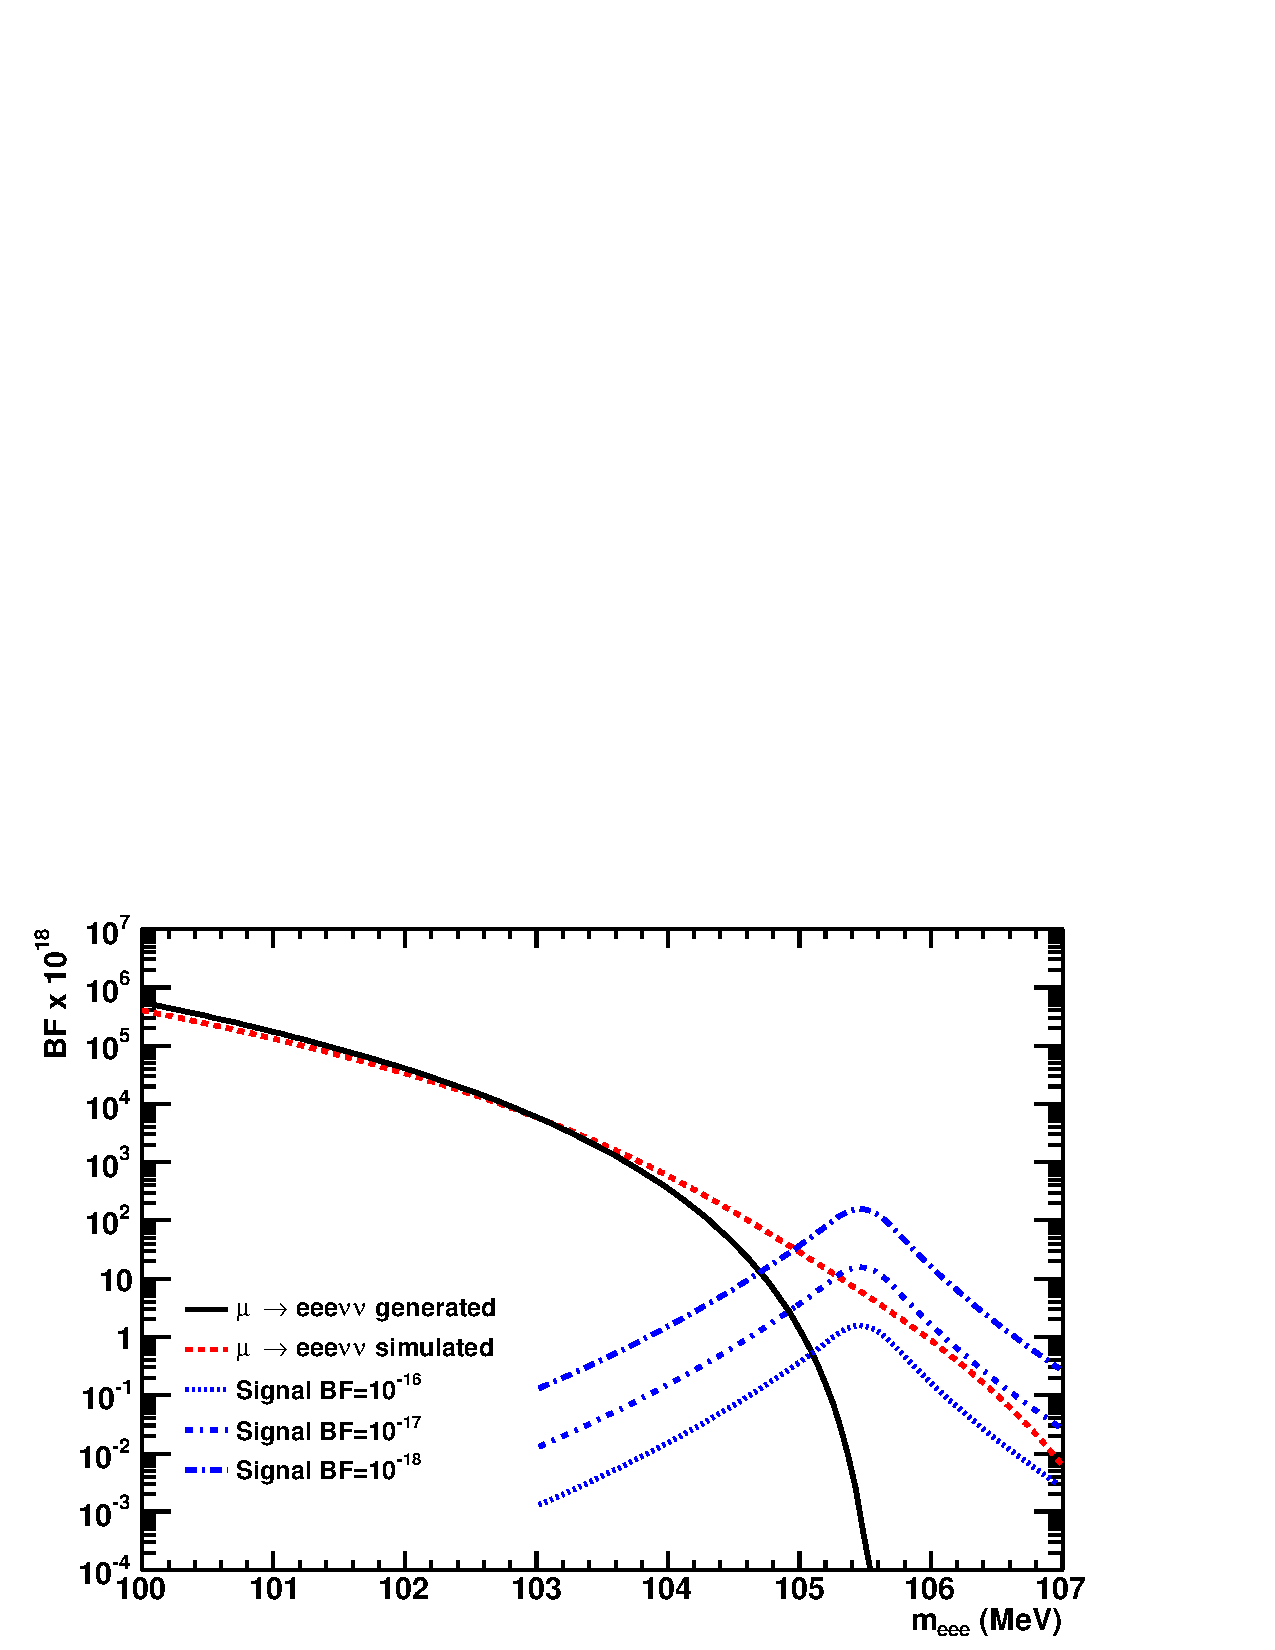
\includegraphics[width=0.45\textwidth]{Figures/mu3e-irr2.pdf}
\end{center}
\caption{The $\mu^+ \rightarrow e^+e^-e^+\nu_e \bar\nu_\mu$ branching fraction before and after convolution with the detector resolution overlaid with signal at different branching 
fractions. Results are shown for 50$\mu$m thick silicon sensors (left) and 30$\mu$m thick silicon sensors (right).}
\label{Fig::mu3e2}
\end{figure}


We consider accidental backgrounds produced by the combination of a Michel decay and a radiative Michel decay (2M$\gamma$ decays), or three simultaneous Michel decays (3M decays), where one the the positron is misreconstructed or produce an electron by interacting with the detector. In both cases, we assume 
the decays occurs within the same pixel in the active target, and during the same time window, set to 250 ps. This yields position and time suppression factors $\delta S = 7.8\times 10^{-7}$ and $\delta t = 2.5\times 10^{-10}$, respectively. 

The number of background events per second can be expressed as:
%
$$N_{2M\gamma} = R_\mu^2 \delta S \delta t BF(\mu^+ \rightarrow e^+ \nu_e \bar\nu_\mu \gamma) BF(\mu^+ \rightarrow e^+ \nu_e \bar\nu_\mu)^2 P(\gamma \rightarrow e^+ e^-)  P_\mu  = 0.33 P_\mu$$
$$N_{3M} = R_\mu^3(\delta S)^2 (\delta t)^2 BF(\mu^+ \rightarrow e^+ \nu_e \bar\nu_\mu)^3 P_\mu = 0.02 P_\mu$$
%
where $P(\gamma \rightarrow e^+ e^-)\sim 0.18\%$ is the probability of photon conversion in the target and $P_\mu$ denotes the probability to reconstruct a muon candidate after all selection criteria are applied. The factors $P_\mu$ are estimated by importance sampling using the differential decay widths given in Ref.~\cite{Kuno:1999jp,Djilkibaev:2008jy}. Values of $P_\mu$ of the order of ${\cal O}(10^{-8})$ (${\cal O}(10^{-9})$) are found for 2M$\gamma$ (3M) decays. Both backgrounds are estimated to be less than one event after a 3-year run period.


In summary, we outline the requirements needed to improve by an order of magnitude the projected sensitivity of the mu3e experiment. The detector setup we study consists of a compact silicon tracker surrounding an active target. We estimate that a stop muon rate of ${\cal O}(8\times 10^{9})$ per second would be required to achieve a SES of $5\times 10^{-18}$ for a 3-year run. Relatively modest improvements on the resolution are needed to maintain the irreducible background at an appropriate level, while an active target proves to be essentially in the reduction of accidental backgrounds. 


